\documentclass[a4paper,12pt,article]{abntex2}

  \usepackage[brazil]{babel}
  \usepackage{fontspec}

  \titulo{Gestão de Resultados de Exames Médicos}
  \autor{Agamenon Lima do Vale}
  \data{\today}

  \usepackage{listings}
    \lstset{language=C}

  \usepackage{graphicx}
\begin{document}
  \imprimirtitulo
  
  \imprimirautor

  \imprimirdata

  \section{Descrição do problema}
    Criar um sistema para armazenar e organizar resultados de exames médicos:
    \begin{itemize}
      \item Armazenar os resultados utilizando uma árvore AVL para garantir ordenação e balanceamento.
      \item Implementar uma funcionalidade de busca eficiente com base em nome ou data.
      \item Realizar estatísticas, como a média dos resultados de um tipo específico de exame, utilizando estruturas auxiliares.
    \end{itemize}
  \section{Explicação da solução implementada}
    O sistema irá trabalhar com três árvores AVL's:
    \begin{enumerate}
      \item Médicos
      \item Pacientes
      \item Exames
    \end{enumerate}
    \subsection{Tipo abstrato de dados}
      Na implementação deste sistema, além das estruturas das árvores AVL, também foi utilizada uma estrutura auxiliar para tratar datas.

      No algoritmo \ref{data} é exibido a estrutura data.

      \begin{lstlisting}[caption=Estrutura para Data, label=data, frame=single, float=h]
        typedef struct Data
        {
          int dia;
          int mes;
          int ano;
        } Data;
      \end{lstlisting}

      Para manipular a estrutura \ref{data}, foi desenvolvida as funções
      \ref{datafunc}.

      \begin{lstlisting}[float=h, caption=Funções para a manipulação da estrutura Data, label=datafunc, frame=single]
        Data *setData(char data[]);
	Data *setDataInt(int dia, int mes, int ano);
	void printData(Data *data);
	char *getData(Data *data);
      \end{lstlisting}

      A função setData recebe, como argumento, uma string que será convertida em uma estrutura Data. Essa estrutura pode ser criada, também, passando o dia, o mês e o ano para a função 
      setDataInt. Para converter uma estrutura Data para string, utiliza-se a função getData.

      A estrutura para médico é exibida em \ref{medicoestrutura}, enquanto em \ref{pacienteestrutura} mostra a estrutura para pacientes e \ref{exameestrutura} visualisa a estrutura
      de exames.

      \begin{lstlisting}[float=h, frame=single, label=medicoestrutura, caption=Estrutura para o objeto médicos]
        typedef struct Medico
        {
          int crm;
          char name[100];
          char especialidade[30];
          char uf[4];
          char celular[15];
          char email[100];
          int height;
          struct Medico *left;
          struct Medico *right;
        } Medico;
      \end{lstlisting}

      \begin{lstlisting}[float=h, frame=single, label=pacienteestrutura, caption=Estrutura para o objeto pacientes]
        typedef struct Paciente
        {
          int id;
          char name[100];
          struct Data *dtNascimento;
          char celular[15];
          char email[100];
          int height;
          struct Paciente *left;
          struct Paciente *right;
        } Paciente;
      \end{lstlisting}
      
      \begin{lstlisting}[float=h, frame=single, label=exameestrutura, caption=Estrutura para o objeto exames]
        typedef struct Exame
        {
          int id;
          char nome[100];
          int idPaciente;
          int crm;
          struct Data *dtRealizacao;
          float resultado;
          int height;
          struct Exame *left;
          struct Exame *right;
        } Exame;
      \end{lstlisting}

    \subsection{Exemplos de execução do programa}

      A figura \ref{menuprincipal} é o menu principal do sistema.

      \begin{figure}[h]
        \centering
        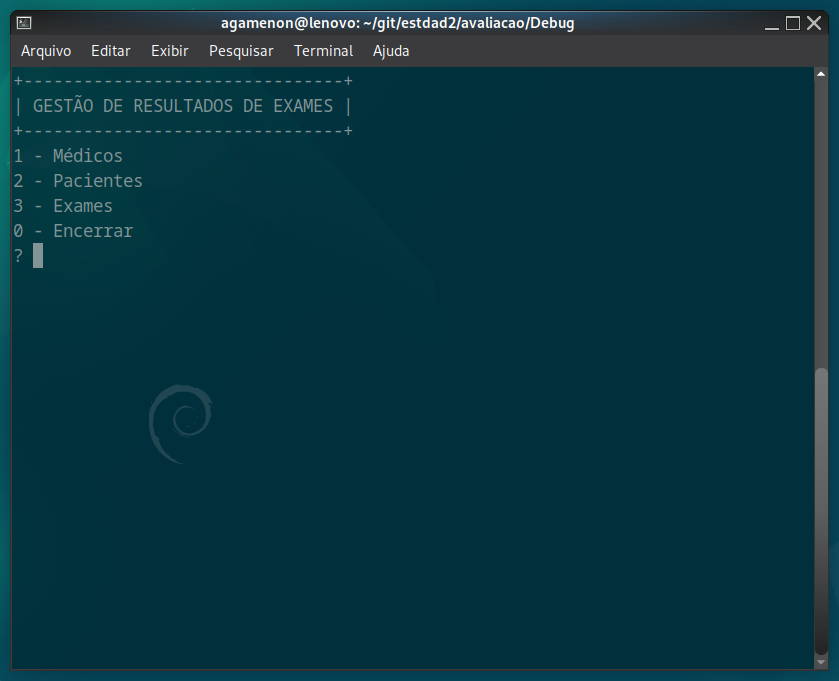
\includegraphics[scale=0.25]{./fig/menuprincipal}
        \caption{Menu principal do sistema}
        \label{menuprincipal}
      \end{figure}

      Na figura \ref{cadastromedico} temos o cadastro de um novo médico no sistema.
      
      \begin{figure}[h]
        \centering
        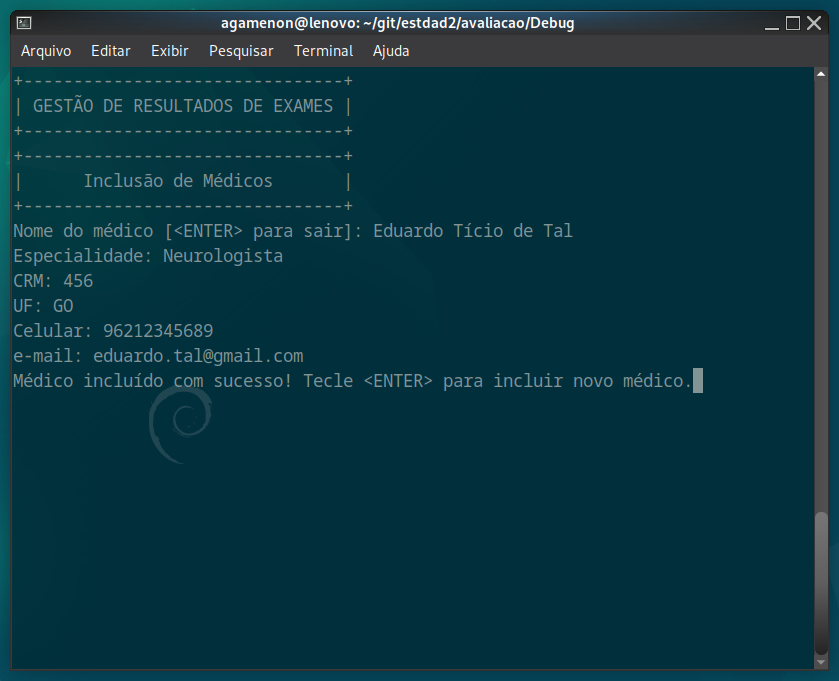
\includegraphics[scale=0.25]{./fig/cadastromedico}
        \caption{Um novo médico sendo cadastrado}
        \label{cadastromedico}
      \end{figure}

      O menu de exames (figura \ref{menuexames}) nos permite diversas listagens de exames.

      \begin{figure}[h]
        \centering
        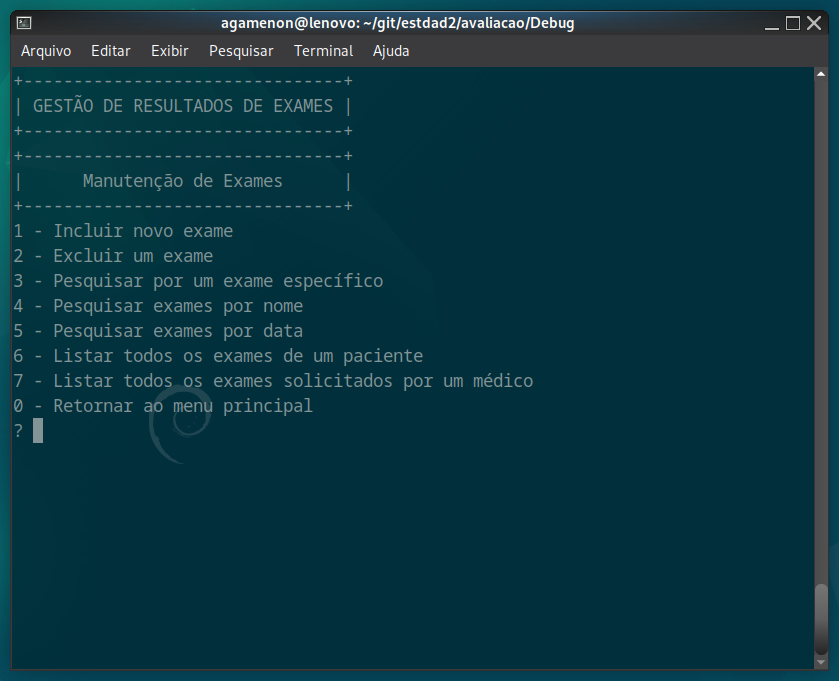
\includegraphics[scale=0.25]{./fig/menuexames}
        \caption{Opções possíveis para o gerenciamento de exames.}
        \label{menuexames}
      \end{figure}

      Um exemplo de listagens de exames solicitados por um médico é visualizado na figura \ref{relacaoexames}.

      \begin{figure}[h]
        \centering
        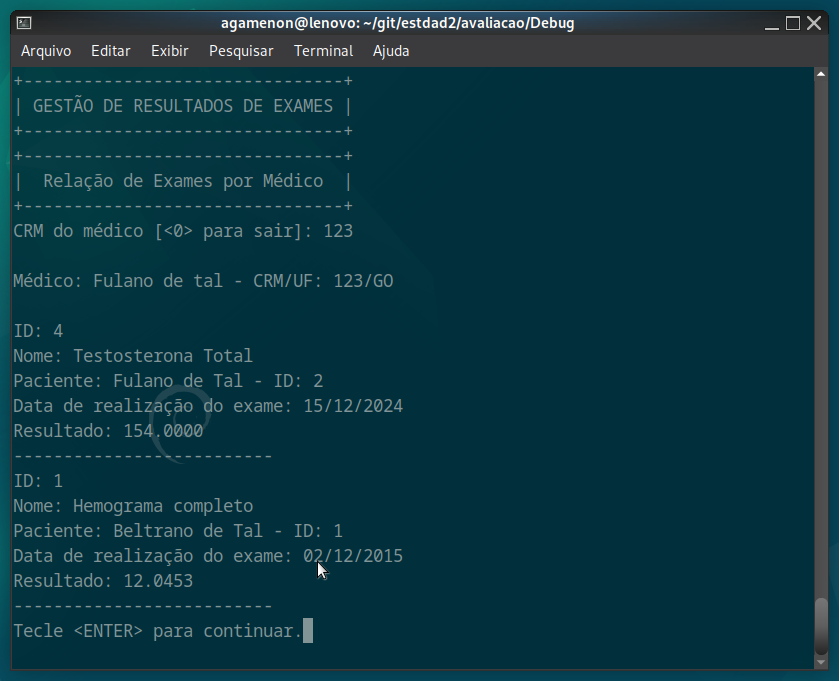
\includegraphics[scale=0.25]{./fig/listaexames}
        \caption{Um exemplo de uma listagem de exames solicitados por um médico.}
        \label{relacaoexames}
      \end{figure}

\end{document}
